\section{Introduction}

Speculative bubbles, since at least the early 18th century South Sea Bubble are perceived \footnote{\cite{garber2001famous} pp 127-31 for references, a particularly is \cite{temin2004riding} a case study of a well-informed investor in the South Sea bubble that knew that a bubble was in progress and that it invested knowingly in the bubble, and found that it was profitable to ride the bubble. } to periodically take over markets. %not quite what he says; fundamentals driven then morals story.
The public notoriety of Bitcoin and the massive price increases and their associated publicity  lead to an explosion of attempts to create ``the next bitcoin'' often referred to as ``cryptocurrencies'' or ``coins'', and a vibrant set of exchanges where these are traded, either for each other or money.
The majority of these coins have no viable uses, and their markets would appear driven largely by speculation.
Many of them appear to be nothing but attempts at turning a quick profit from inflating the implied valuation of a coin shortly after creating it.
This is driven by the extremely low cost and effort required to create a new coin, with most being minimal changes to parameters and branding of a pre-existing codebase.
Those who make and trade these coins communicate largely online, and much of their activity is concentrated on public forums, while price and volume data from their exchanges is freely available and widely aggregated.


We present a novel dataset based on the Bitcoin Talk forum that allows us to identify the introducers of each coin and build measures of their position in the network based on which users have engaged with their threads in the forum before the coin is announced.
While speculation during bubbles as a social process that has been theoretically studied \cite{abolafia1988enacting, earl2007decision, bakker2010social, harras2011grow}, an exaustive dataset on the social network underpinning them has not been previously available.
Our most conservative dataset identifies 376 coins that are announced by users of the forum and which can be mapped to price and volume data from exchanges.
By considering the community structure that exists in the forum before a coin is introduced we are able to predict part of the variation in both the severity and magnitude of the resulting bubble: our best model explains a quarter of the variation in the severity and around two percent of the magnitude of the bubbles in our of sample cross validation. 
The main driver of our explanatory power is the centrality of a user in the directed network derived from 
We also collect the set of prices and traded volumes across the cryptocurrencies that are introduced in the discussions on the forums, and construct measures of both the intensity (aka severity, for each dollar invested at the peak what could be recovered on average) and the magnitude (how many dollars or bitcoins where nominally traded in the asset).

\includegraphics{volume1}

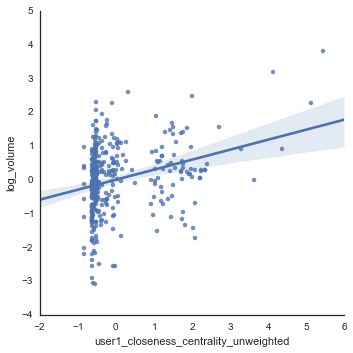
\includegraphics{volume2}

This allows us to evaluate the predictive power of the features of the node in our constructed network that corresponds to the user who first introduces the coin. 
While the magnitude of the assets traded is small relative to most financial and commodity markets, it is much larger than even the most lavishly funded experimenter could hope for.
Furthermore, the rich market structure that surrounds (some 45 exchanges appear on the dataset, ranging in credibility from VC backed and registered in the US, to anonymous and mysteriously run) provides a rich source of institutional variation with extremely open data, a striking contrast to most financial or commodities market trade level data. 
x
The evidence based uncovered by “— traces of their communicative interactions as they work out their thoughts about matters of common concern” 

\begin{quote}
"Bitcoin is a purely online virtual currency, unbacked by either physical commodities or sovereign obligation; instead, it relies on a combination of cryptographic protection and a peer-to-peer protocol for witnessing settlements. Consequently, Bitcoin has the unintuitive property that while the ownership of money is implicitly anonymous, its flow is globally visible. In this paper we explore this unique characteristic further, using heuristic clustering to group Bitcoin wallets based on evidence of shared authority, and then using re-identification attacks (i.e., empirical purchasing of goods and services) to classify the operators of those clusters. From this analysis, we characterize longitudinal changes in the Bitcoin market, the stresses these changes are placing on the system, and the challenges for those seeking to use Bitcoin for criminal or fraudulent purposes at scale." 
\end{quote} 
\cite{meiklejohn2013fistful}

While states can create the demand required for a currency system to run by compelling tax payment in it (for a recent example), non state sponsored currencies must find some other ways of creating demand.
The initial market for which bitcoin has been used (prices denominated in it, transactions only in it) was drug sales.\footnote{A overview of the different drug marketplaces and estimated transaction volumes can be found in \cite{soska2015measuring}. To the best of the authors knowledge no other sector beyond speculation has even remotely substantial volume at present; a very primitive form of unregulated gambling Satoshi Dice, did for a brief pointing the past)   }
Since the cost of producing a new coin is effectively zero, new currencies have thus been floated with every single drug name possible. Many chains can claim to the same name, so exchanges with volume (since speculation is the only possible use of almost all of the coins) become de-facto arbitrators of who has a minimally viable claim.\footnote{While it is theoretically possible to engage in a distributed protocol to exchange between two cryptocurrencies, see part II of lecture 10 in \cite{princeton10}}





%Methodologically the free parameters in the way we do the weights on the weighted graph  is horrible, a millon free parameters get introduced. follow up work for another paper: do some unsupervised feature learning over the dam forums threads to build the network; use some internal validity metric . Find political way of saying this in future work.

